\section{Property Inference Attacke}\label{sec:property_inference}

Bei der sogenannten Property Inference Attacke versucht ein Angreifer, bestimmte Eigenschaften über die Daten eines Modells herauszufinden, welche nur indirekt von einem Modell gelernt wurden und auch nicht bewusst veröffentlicht wurden \cite{P-80}.

Ateniese et al. \cite{P-80} zeigten erstmals, wie so ein Angriff bei Machine Learning Modellen ,wie einer Support Vektor Maschine, funktionieren kann.
Es wird gezeigt, dass es möglich ist, herauszufinden, ob das angegriffene Modell eine bestimmte Eigenschaft der Daten gelernt hat. 
Um dies zu erreichen, konstruiert der Angreifer mehrere Datensätze, in denen die zu untersuchende Eigenschaft vorhanden ist oder nicht. 
Anschließend werden diese Datensätze genutzt, um verschiedene Modelle zu trainieren, welche die gleiche Architektur wie das angegriffene Modell nachbilden.
Der Schlüssel dieser Methode ist es, nun einen Meta-Klassifikator mit diesen Modellen zu trainieren.
Bei Meta-Klassifikatoren handelt es sich um Modelle, welche aus anderen Modellen lernen. 
Konkret werden hierbei die Parameter der Modelle als Input genutzt, um vorherzusagen, ob die Trainingsdaten die zu untersuchende Eigenschaft besitzen. 
Dies ist möglich, da alle Modelle, das angegriffene Modell und die vom Angreifer trainierten Modelle, die gleiche Architektur haben und dadurch auch zum gleichen Format transformiert werden können.
Ateniese et al. konnten mit diesem Angriff zeigen, dass es möglich ist, herauszufinden, ob ein Sprachmodell mit Daten der Eigenschaft \dq Sprecher mit indischem Dialekt \dq trainiert wurde. 

\begin{figure}[!htb]
    \centering
    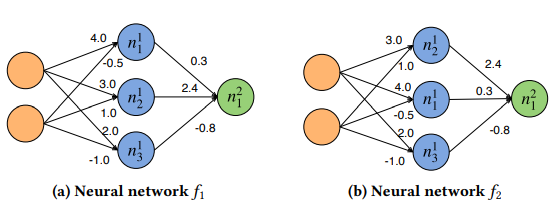
\includegraphics[width=12cm]{figures/permutation_invariance}
    \caption{Permutation eines Neuronalen Netzes \cite{P-11}}
    \label{fig:permutation_invariance}
\end{figure} 

Die Methode von Ateniese et al. \cite{P-80} ist auf diverse Machine Learning Modelle wie Hidden Markov Modelle oder Support Vektor Maschinen ausgelegt, weshalb diese bei Neuronalen Netzen nicht sonderlich gut funktioniert. 
Ganju et al. \cite{P-11} passten den Angriff auf Neuronale Netze an, indem zwei geeignete Repräsentation für diese Art von Modellen genutzt werden kann.
Die erste Repräsentation eines Neuronalen Netz basiert auf der Eigenschaft von Neuronalen Netzen, dass die Reihenfolge der Neuronen vertauscht werden kann. 
Abbildung \ref{fig:permutation_invariance} zeigt zwei Neuronale Netze, bei denen die Reihenfolge der Knoten in der ersten Hidden Layer vertauscht ist, jedoch das Modell die gleiche Funktion berechnet.
Diese Eigenschaft kann nun genutzt werden, um jede Schicht zu sortieren und dadurch eine einheitliche Matrix für Permutationen des gleichen Modells zu erhalten.

Die zweite Repräsentation beruht darauf, die Schichten eines Neuronalen Netzes nicht als Vektor darzustellen.
Im Gegensatz zu einem Vektor hat ein Set keine feste Reihenfolge oder Ordnung, sondern ist lediglich eine Menge von Objekten, bzw. hier von Knoten.
Dies sorgt ebenfalls dafür, dass Permutationen des gleichen Modells, in das gleiche Format übertragen werden können.
Ganju et al. \cite{P-11} zeigen anhand des MNIST Datensatzes, dass beide Repräsentationsformen die Accuracy des Meta-Klassifikators erhöhen können.

Gopinath et al. \cite{P-12} zeigen, dass viele Informationen eines Neuronalen Netzes in der Aktivierung der Neuronen steckt. 
Dabei reicht es, einen Wert in \textbf{on} und \textbf{off} zu unterteilen, wobei on einem Wert > 0 entspricht. 
Gopinath et al. \cite{P-12} nutzten diese Darstellung für eine gutwillige Informationsgewinnung über ein Modell, jedoch könnte die Darstellung auch für Property Inference Angriffe genutzt werden.